%% -*- coding:utf-8 -*- 
\documentclass[14pt,a4paper]{article} 
\input preamble.tex
\title{Probability paradoxes}
\author{Ivan Murashko}
\date{}
\begin{document}

\maketitle
\tableofcontents

\section*{Introduction}
The goal for the article is to demonstrate several paradoxes that are
related to probability theory and how can they can be solved.

\section{Base definitions of probability theory}
I am going to provide several definitions. I will give the both formal
and informal definitions and show how they are related each other.

We will start with the simplest example. 
\begin{example}
\label{ex:initial}
In the example we have (see \cref{fig:simpleprobability}) $N=5$ balls.
There are $N_G = 2$ green balls and $N_R$ red balls. I.e. $N = N_G +
N_R$.  
\begin{figure}[H]
  \centering
  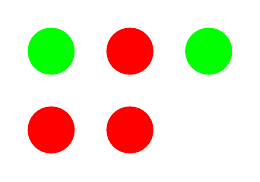
\begin{tikzpicture}[ele/.style={fill=black,circle,minimum
        width=.8pt,inner sep=1pt},every fit/.style={ellipse,draw,inner
        sep=-2pt}]
    \tikzstyle{element}=[circle,fill=black!25,minimum size=17pt,inner sep=0pt]

    \node[element, color=green] at (0,1) {};
    \node[element, color=red] at (1,1) {};
    \node[element, color=green] at (2,1) {};
    \node[element, color=red] at (0,0) {};
    \node[element, color=red] at (1,0) {};


  \end{tikzpicture}
  \caption{Probability example}
  \label{fig:simpleprobability}
\end{figure}

We can define the probability to get green ball as
\[
P_G = \frac{N_G}{N} = \frac{2}{5}
\]
and the probability to get red ball as
\[
P_R = \frac{N_R}{N} = \frac{3}{5}.
\]
We can get only a red or a green ball and 
\[
P_G + P_R = 1.
\]
\end{example}

Now we are ready to give several formal definitions. 
\begin{definition}[$\sigma$ algebra]
Let $\Omega$ is a set then a collection $\mathcal{F}$ of sub sets of
$\Omega$ is called $\sigma$ algebra if the following conditions are
satisfied:
\begin{enumerate}
\item $\mathcal{F}$ contains $\Omega$: $\Omega \in \mathcal{F}$
\item TBD
\item TBD
\end{enumerate} 
\end{definition}

In our \cref{ex:initial}, $\sigma$ algebra is a collection of any
balls. 

\begin{figure}
  \centering
  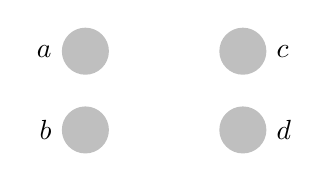
\begin{tikzpicture}[ele/.style={fill=black,circle,minimum
        width=.8pt,inner sep=1pt},every fit/.style={ellipse,draw,inner
        sep=-2pt}]

    % the texts
    \tikzstyle{element}=[circle,fill=black!25,minimum size=17pt,inner
      sep=0pt]

    \node[element,label=left:$a$] (a) at (0,2) {};    
    \node[element,label=left:$b$] (b) at (0,1) {};    
    \node[element,label=right:$c$] (c) at (2,2) {};
    \node[element,label=right:$d$] (d) at (2,1) {};
    
  \end{tikzpicture}
  \caption{Probability space. It consists of elementary events: $a$,
    $b$, $c$ and $d$, each
    of them has equal probability $p_{a,b,c,d} = \frac{1}{4}$}
  \label{fig:probabilityspace}
\end{figure}

\begin{figure}
  \centering
  
\begin{tikzpicture}[ele/.style={fill=black,circle,minimum
        width=.8pt,inner sep=1pt},every fit/.style={ellipse,draw,inner
        sep=-2pt}]
    \tikzstyle{element}=[circle,fill=black!25,minimum size=17pt,inner sep=0pt]

    \node[element,top color=green, bottom color=red] at (0,1) {};
    \node[element,top color=green, bottom color=red] at (1,1) {};
    \node[element,top color=green, bottom color=red] at (2,1) {};
    \node[element,top color=red, bottom color=blue] at (0,0) {};
    \node[element,top color=red, bottom color=blue] at (1,0) {};
    \node[element,top color=green, bottom color=blue] at (2,0) {};


  \end{tikzpicture}
  \caption{Condition probability. Original probability space. $P(R) =
    \frac{5}{6}$, $P(B) = \frac{3}{6}$, $P(G) = \frac{4}{6}$
  }
  \label{fig:condprobability}
\end{figure}

\begin{figure}
  \centering
  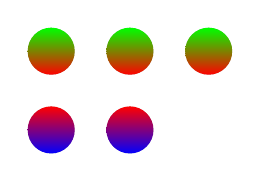
\begin{tikzpicture}[ele/.style={fill=black,circle,minimum
        width=.8pt,inner sep=1pt},every fit/.style={ellipse,draw,inner
        sep=-2pt}]
    \tikzstyle{element}=[circle,fill=black!25,minimum size=17pt,inner sep=0pt]

    \node[element,top color=green, bottom color=red] at (0,1) {};
    \node[element,top color=green, bottom color=red] at (1,1) {};
    \node[element,top color=green, bottom color=red] at (2,1) {};
    \node[element,top color=red, bottom color=blue] at (0,0) {};
    \node[element,top color=red, bottom color=blue] at (1,0) {};


  \end{tikzpicture}
  \caption{Condition probability. $P(G|R) = \frac{3}{5}$, $P(B|R) = \frac{2}{5}$}
  \label{fig:condprobability_red}
\end{figure}

\begin{figure}
  \centering
  
\begin{tikzpicture}[ele/.style={fill=black,circle,minimum
        width=.8pt,inner sep=1pt},every fit/.style={ellipse,draw,inner
        sep=-2pt}]
    \tikzstyle{element}=[circle,fill=black!25,minimum size=17pt,inner sep=0pt]

    \node[element,top color=red, bottom color=blue] at (0,0) {};
    \node[element,top color=red, bottom color=blue] at (1,0) {};
    \node[element,top color=green, bottom color=blue] at (2,0) {};


  \end{tikzpicture}
  \caption{Condition probability. $P(R|B) = \frac{2}{3}$, $P(G|B) = \frac{1}{3}$}
  \label{fig:condprobability_blue}
\end{figure}

\begin{figure}
  \centering
  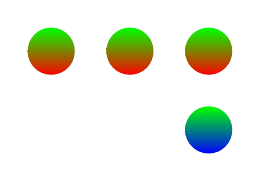
\begin{tikzpicture}[ele/.style={fill=black,circle,minimum
        width=.8pt,inner sep=1pt},every fit/.style={ellipse,draw,inner
        sep=-2pt}]
    \tikzstyle{element}=[circle,fill=black!25,minimum size=17pt,inner sep=0pt]

    \node[element,top color=green, bottom color=red] at (0,1) {};
    \node[element,top color=green, bottom color=red] at (1,1) {};
    \node[element,top color=green, bottom color=red] at (2,1) {};
    \node[element,top color=green, bottom color=blue] at (2,0) {};


  \end{tikzpicture}
  \caption{Condition probability. $P(B|G) = \frac{1}{4}$, $P(R|G) = \frac{3}{4}$}
  \label{fig:condprobability_green}
\end{figure}


TBD \cite{bib:kolmogorov74basic}

\section{Monty Hall problem}
TBD

\section{Waiting time on a bus stop}
TBD

\bibliographystyle{gost780s}  
\bibliography{probability}     


\end{document}
